\section{Bayes' theorem}

Bayes' theorem describes the probability of an event to occur, depending on the prior knowledge of conditions related to the event \citep{bayesBasic}. 
\begin{equation}
\label{eqn:bayesianTheorem}
P(A|B) = \frac{P(B|A)P(A)}{P(B)}.
\end{equation}
P(A|B) is the posterior probability of A given that B is true. P(B|A) is called conditional probability of B given A being true. P(A) is the prior probability, the probability of A occurring without any additional information. Finally P(B) is the marginal probability of B without any given condition. This theorem is often used for Bayesian inference where it expresses how a belief, which is represented as probability changes due to related evidence.	

\section{Bayesian inference}
\label{section:bayesianInference}

Bayesian inference is a process of data analysis to calculate the probability of a hypothesis depending on the available related evidence. As over time more and more evidence becomes available the probabilities can be updated yielding a more sophisticated view on the hypothesis. It is given, according to Bayes' theorem, by
\begin{equation}
\label{eqn:bayesianInference}
P(H|E) = \frac{P(E|H)P(H)}{P(E)},
\end{equation}
where H represents a hypothesis and E some related evidence. P(H|E) is the posterior probability which signifies the probability of the hypothesis after the evidence was observed. P(E|H) is called likelihood and it is the probability of observing the evidence 	given the hypothesis. It is a measure of the compatibility of the observed evidence with the given hypothesis. P(H) is the prior probability which is the probability of the hypothesis before any evidence is considered or obtained. P(E) is called marginal likelihood that represents the probability of the evidence being observed. However it is the same independent of the chosen hypothesis. Thus, it is not factored in when comparing different hypotheses.
Bayesian inference can be applied to the "face in shadow" example of Section \ref{section:feedbackInVisualCortex}. There a neuron in V1 sees a small part of the visual field and signals if it sees an edge or not. At first it has the evidence of the observed pixels available and from it can calculate the likelihood that an edge is present. At first it has no prior knowledge of how probable an edge being present is, meaning that the prior probabilities for there being an edge or no edge are equal. With that likelihood and the prior probabilities it can conclude the posterior probability for the hypothesis "there is an edge" and decides that there is no edge.
Later the inferior temporal cortex determines that there is a face in the picture and feeds this information back to V1. This influences the prior probabilities and changes the posterior probability in a way that the V1 neuron starts to see the hypothesis that there is an edge as more likely, in order to complete the contour of the face. 
We now define X as a binary random vector of the visual input, Y as a multinomial variable of the output of V1 and Z as a multinomial variable of the feedback of the inferior temporal cortex.
When plugging these variables into Equation \ref{eqn:bayesianInference} with the posterior given by $P(Y|X,Z)$, the likelihood given by $P(X|Y)$ and the prior given by $P(Y|Z)$ we get
\begin{equation}
\label{eqn:pYvorausgesetztXUndZ}
P(Y = k|X = x, Z = j) = \frac{P(X=x|Y=k)P(Y = k|Z = j)}{\Sigma_{k'}P(X=x|Y=k')P(Y=k'|Z=j)}.
\end{equation}

\section{Network model}

The network model used for the experiments in this thesis was taken from \citet{nessler} and expanded by an additional layer to include some hierarchical feedback information.

\paragraph{Neuron model}
As in \citet{nessler} the input neurons $x_1,...,x_n$ are firing according to a poisson process with an average firing rate $f_{input}$ when active and with 0 Hz when in an inactive state. The input neurons receive a binary input, for example a black or white pixel of an image. The excitatory post synaptic potentials (EPSPs) $x_i(t)$ that these neurons produce can be seen in Figure \ref{fig:XSpike}. A double exponential kernel was used to generate the EPSP. The kernel has a time constant for the rise of the signal $\tau_{rise}$  and a time constant for the decay of the signal $\tau_{decay}$. The addition of the time step size $\delta t$ was necessary to get the time t at the end of the current simulation step. $t_f$ is the time at which the spike of $x_i$ occurred
\begin{equation}
\label{eqn:EPSP}
x_i(t) = e^{-(t + \delta t - t_f) / \tau_{decay}} - e^{-(t + \delta t - t_f) / \tau_{rise}}.
\end{equation}
Analogously the EPSP of the prior neurons $z_j(t)$ are given by
\begin{equation}
\label{eqn:EPSPPrior}
z_j(t) = e^{-(t + \delta t - t_f) / \tau_{decay}} - e^{-(t + \delta t - t_f) / \tau_{rise}}.
\end{equation}

\begin{figure}
  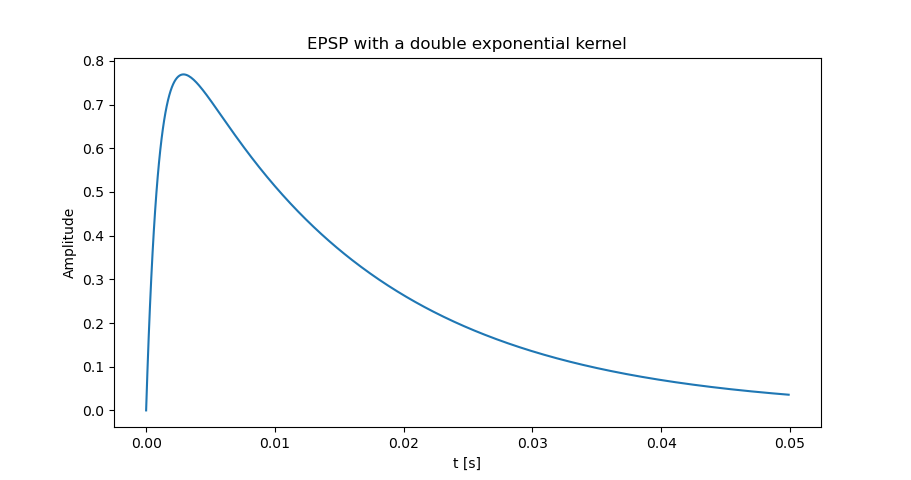
\includegraphics[width=\linewidth]{figures/XSpike.png}
  \caption{Form of an excitatory post synaptic potential generated by an input neuron over time. A double exponential kernel was used to generate this signal. These signals are fed to the next layer of the network. }
  \label{fig:XSpike}
\end{figure}

The membrane potential $u_k$ of each output neuron is calculated by multiplying the EPSP of each input neuron times the input weight $w^{I}_{ki}$ of the connection between them, plus the EPSP of each prior neuron times the prior weight $w^{P}_{kj}$
\begin{equation}
\label{eqn:uk}
u_k(t) = \sum_{i=1}^N w^{I}_{ki} \cdot x_i(t) + \sum_{j=1}^J w^{P}_{kj} \cdot z_j(t).
\end{equation}

In \citet{nessler} each output neuron $y_k$ also had an intrinsic excitability $w_{k0}$ which was learned for each neuron. For the experiments of this thesis however it was omitted, as the different classes of  input images were equally likely, thus the intrinsic excitabilities of the output neurons would all end up being equal to each other.

The output neurons are modelled in a winner-takes-all (WTA) circuit. The WTA behaviour was implemented via an adaptive inhibition signal. The adaptive inhibition is used to regulate the membrane potentials of the output neurons so that all of them together fire with a total firing rate $R(t) = 200 Hz$ on average. Due to that there never is a time window in which no output neuron may fire. However, it is unlikely for an output neuron to fire right after another output neuron has fired.

The inhibition signal was chosen to depend on the current membrane potential of the output neurons. 
Solving Equation \ref{eqn:R} for I(t) yields
\begin{equation}
\label{}
R(t) = \frac{ \sum_{k=1}^K e^{u_k(t)}}{e^{I(t)}}
\end{equation}
\begin{equation}
\label{}
e^{I(t)} = \frac{\sum_{k=1}^K e^{u_k(t)}}{R(t)}
\end{equation}
\begin{equation}
\label{}
I(t) = \ln{ \frac{ \sum_{k=1}^K e^{u_k(t)}}{R(t)}}
\end{equation}
\begin{equation}
\label{eqn:I(t)}
I(t) =  - \ln{R(t)} + \ln{  \sum_{k=1}^K e^{u_k(t)}}.
\end{equation}

\citet{nessler} defined that the firing probability of an output neuron  $y_k$ is exponentially proportional to its membrane potential $u_k$ minus the received inhibition $I(t)$
\begin{equation}
\label{eqn:pVonY}
p(y_k \text{ fires at time t}) \propto e^{u_k(t) - I(t)}.
\end{equation}
This stochastic firing model is supported by experimental biological evidence \citep{woDasEHerkommt}. Through this definition the firing rate $r_k(t)$ of an output neuron is then modelled by an inhomogeneous Poisson process as
\begin{equation}
\label{eqn:rk}
r_k(t) = e^{u_k(t) - I(t)}.
\end{equation}
At every timestep of the simulation the inhibition signal I(t) is subtracted from the membrane potential $u_k(t)$ of every output neuron. By that the membrane potentials are altered to always yield a spiking frequency of 200 Hz, regardless if it would be lower or higher without it. This means that the adaptive inhibition signal can also function as an excitatory signal. 

The total firing rate of the output neurons is obtained when summing up the firing rates of all output neurons, yielding 
\begin{equation}
\label{eqn:R}
R(t) = \sum_{k=1}^K e^{u_k(t) - I(t)}.
\end{equation}

The probability of an individual output neuron to fire within a time step $\delta t$ is given by
\begin{equation}
\label{eqn:rkdt}
r_k(t) \delta t.
\end{equation}

The conditional probability $q_k(t)$ that a spike originated from the output neuron $y_k$ is given by
\begin{equation}
\label{eqn:qk}
q_k(t) = \frac{r_k(t) \delta t}{R(t) \delta t} = \frac{e^{u_k(t) - I(t)}}{\sum_{k'=1}^K e^{u_{k'}(t) - I(t)}} = \frac{e^{u_k(t)}}{\sum_{k'=1}^K e^{u_{k'}(t)}}.
\end{equation}
The inhibition term cancels out because all output neurons receive the same inhibition, meaning that it is independent of k.

\paragraph{Spike timing dependent plasticity}
The input weights $w^{I}_{ki}$ between neurons $x_i$ and $y_k$ are updated whenever an output neuron fires. $\sigma$ indicates the time window, after which spikes are no longer considered. If $y_k$ produces a spike all its weights to the input neurons are updated as
\begin{equation}
\label{deltawki}
\Delta w^{I}_{ki} = \begin{dcases*} \lambda \cdot (ce^{-w^{I}_{ki}} - 1) & if $x_{i}$ fired in $ [t^f - \sigma, t^f] $ \\
\lambda \cdot (-1) & \text{if $ x_i $ did not fire in $ [t^f - \sigma, t^f] $, } \end{dcases*}
\end{equation}
where $\lambda$ is the learning rate, the parameter c shifts the weight values, $t^f$ is the time when $y_k$ spiked and $\sigma$ is the time window in which input spikes are considered as "before" an output spike. As the membrane potentials $u_k$ of the output neurons result from the addition of the EPSPs of the input neurons times the corresponding weight, a way to control the average size of u is needed. If u is too small the output neurons will fire too sparsely and if u is too big it will impair the learning process. So to limit u, the size of the weights is controlled via the parameter c. The learning rate $\lambda$ is needed to control the size of each weight update. If it is too big few output neurons will respond to multiple input classes and others will only respond too little or not at all. On the other hand if $\lambda$ is too small the network will learn very slowly and may never converge.
The prior weights $w^{P}_{kj}$ are also updated whenever an output neuron fires, in the same way as $w^{I}_{ki}$
\begin{equation}
\label{deltawkj}
\Delta w^{P}_{kj} = \begin{dcases*} \lambda \cdot (ce^{-w^{P}_{kj}} - 1) & if $z_{j}$ fired in $ [t^f - \sigma, t^f] $ \\
\lambda \cdot (-1) & \text{if $ z_j $ did not fire in $ [t^f - \sigma, t^f] $, } \end{dcases*}
\end{equation}

\paragraph{Network architecture}
Each pixel of an input image was connected to two neurons. The first of these neurons is in an active state when the pixel is black and in an inactive state otherwise. The second neuron expresses the opposite behaviour. As a consequence the network needs ($width \cdot height \cdot 2$) excitatory input neurons $x_1,...,x_N$. These input neurons are fully connected to the excitatory output neurons $y_1,...,y_K$. This means that every input neuron $x_i$ is connected to each output neuron $y_k$. 
To simulate the feedback from the inferior temporal cortex prior neurons $z_1,...,z_J$ were added to the network. The prior neurons were also fully connected to the output neurons. A visualization of the network architecture can be seen in Figure \ref{fig:networkArchitecture}.

\begin{figure}
  \label{fig:networkArchitecture}
  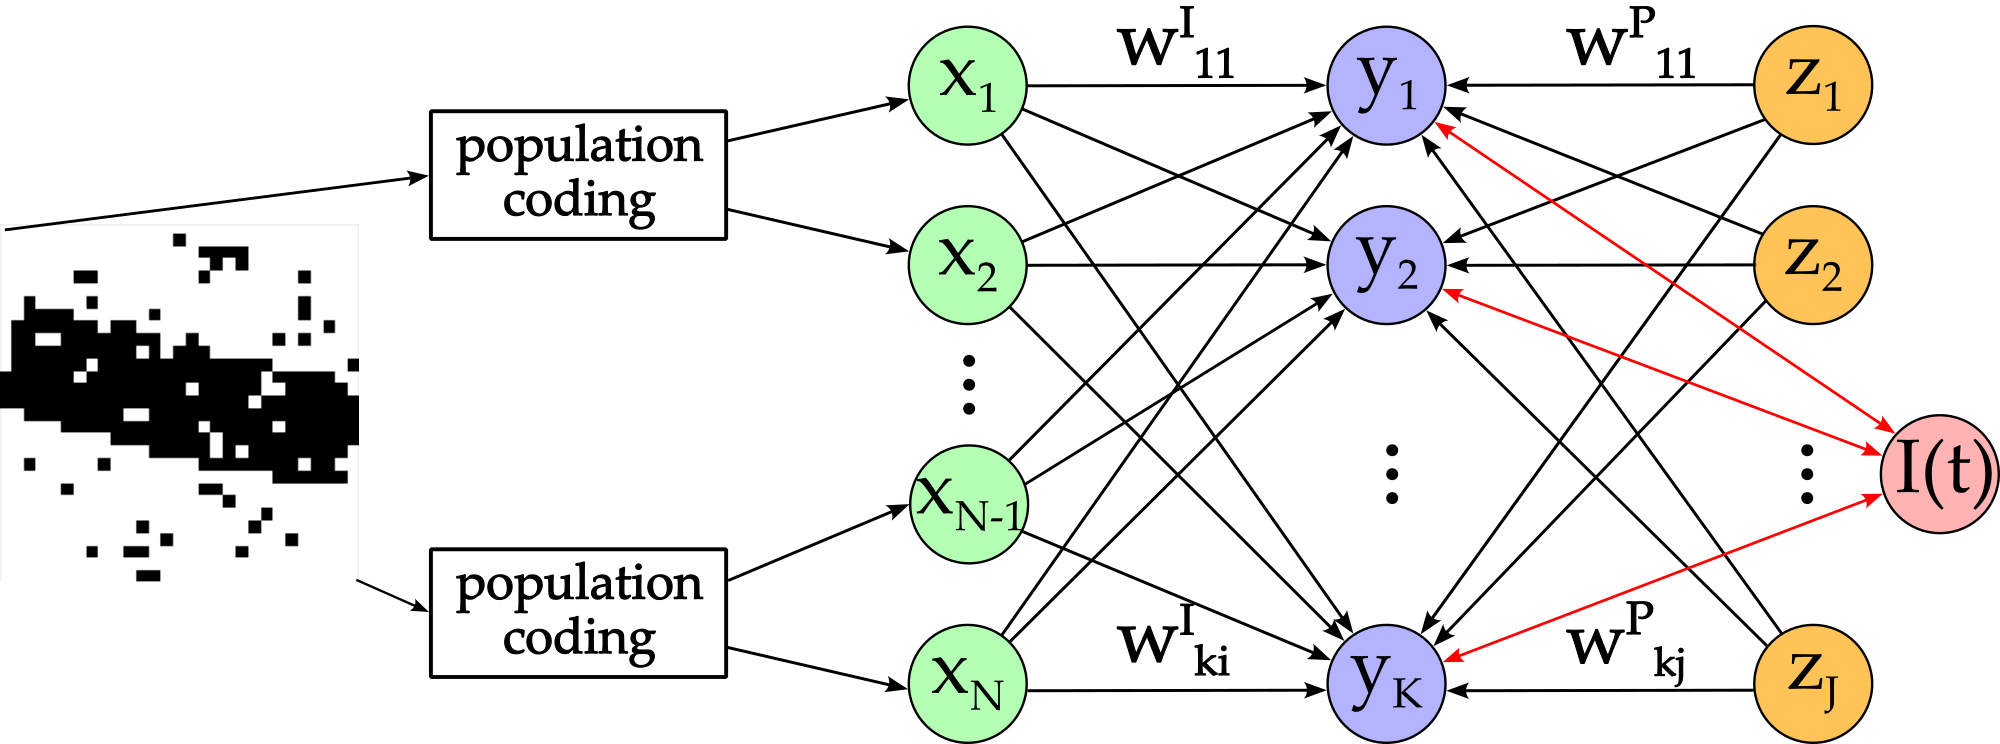
\includegraphics[width=\linewidth]{figures/networkPlan.png}
  \caption{Architecture of the network.}
\end{figure}

\section{Mathematical link between the spiking Winner-Take-All network model and Bayesian inference}
\label{linkNetworkBayes}

\citet{nessler} hypothesized that the ensemble of weights of a neuron can be understood as a generative model. They further claimed that every synaptic weight, due to STDP-induced changes,  converges stochastically to the log of the conditional probability that the presynaptic neuron has fired just before the postsynaptic neuron, given that the postsynaptic neuron fires. This connection is given by
\begin{equation}
\label{eqn:weightProbLink}
 w^{I}_{ki} = log(p(x_i = 1 | y_k = 1))
\end{equation}
an will be analysed in Section \ref{section:1D}.
Furthermore they claimed that in a Bayesian inference context every input spike provides evidence for an observed variable and every output spike represents one stochastic sample from the posterior distribution over hidden causes, which are encoded in the circuit. 

To show the connection between the spiking Winner-Take-All network model and Bayesian inference it will be shown that the posterior probability of Bayesian inference given in Equation \ref{eqn:pYvorausgesetztXUndZ} is equal to the relative firing probability $q_k(t)$, given in Equation \ref{eqn:qk}.

As explained in Section \ref{section:bayesianInference} the visual input, modelled by the input neurons can be thought of as the Bayesian likelihood and the feedback, modelled by the prior neurons, as the Bayesian prior. As defined in Equation \ref{eqn:pVonY} the firing probability of an output neuron is proportional to the exponent of its membrane potential minus the inhibition. To obtain the Bayesian likelihood and prior we first split the membrane potential into the contributions of the input and prior neurons. The first part that signifies the contribution of the input neurons is given by
\begin{equation}
e^{u_x} = e^{\sum_{i=1}^N w^{I}_{ki} \cdot x_i(t)}.
\end{equation}
The second part gives the contribution of the prior neurons as
\begin{equation}
e^{u_z} = e^{\sum_{j=1}^J w^{P}_{kj} \cdot z_j(t)}.
\end{equation}

These two parts can be seen as two partial membrane potentials. By inserting each of them into Equation \ref{eqn:pVonY} we get the likelihood
\begin{equation}
P(X|Y) = e^{u_x - I(t)}.
\end{equation}
and the prior
\begin{equation}
P(Y|Z) = e^{u_z - I(t)}.
\end{equation}

When inserting the likelihood and the prior into Equation \ref{eqn:pYvorausgesetztXUndZ} we get

\begin{equation}
\begin{split}
P(Y=k|X=x,Z=j) &= \frac{e^{\sum_{i=1}^N w{i}_{ki} \cdot x_i(t) - I(t)} \cdot e^{\sum_{j=1}^J w^{P}_{kj} \cdot z_j(t) - I(t)}}{\sum_{k'=1}^K  e^{\sum_{i=1}^N w^{I}_{k'i} \cdot x_i(t) - I(t)} \cdot e^{\sum_{j=1}^J w^{P}_{k'j} \cdot z_j(t) - I(t)}}\\
&= \frac{e^{-I(t) \cdot N + \sum_{i=1}^N w^{I}_{ki} \cdot x_i(t)} \cdot e^{-I(t) \cdot J + \sum_{j=1}^J w^{P}_{kj} \cdot z_j(t)}}{\sum_{k'=1}^K  e^{-I(t) \cdot N + \sum_{i=1}^N w^{I}_{k'i} \cdot x_i(t)} \cdot e^{-I(t) \cdot J + \sum_{j=1}^J w^{P}_{k'j} \cdot z_j(t)}}\\
&= \frac{e^{-I(t) \cdot N} \cdot e^{\sum_{i=1}^N w^{I}_{ki} \cdot x_i(t)} \cdot e^{-I(t) \cdot J} \cdot e^{\sum_{j=1}^J w^{P}_{kj} \cdot z_j(t)}}{e^{-I(t) \cdot N} \cdot e^{-I(t) \cdot J} \cdot \sum_{k'=1}^K  e^{\sum_{i=1}^N w^{I}_{k'i} \cdot x_i(t)} \cdot e^{\sum_{j=1}^J w^{P}_{k'j} \cdot z_j(t)}}\\
&= \frac{e^{\sum_{i=1}^N w^{I}_{ki} \cdot x_i(t) + \sum_{j=1}^J w^{P}_{kj} \cdot z_j(t)}}{\sum_{k'=1}^K  e^{\sum_{i=1}^N w^{I}_{k'i} \cdot x_i(t) + \sum_{j=1}^J w^{P}_{k'j} \cdot z_j(t)}}\\
&= \frac{e^{U_k(t)}}{\sum_{k'=1}^K e^{U_k'(t)}}\\
&= q_k(t)
\end{split}
\end{equation}


